\documentclass[12pt]{article}
\title{ DATA MINING (CSCI-B 565)  \\
Assignment $1$ \\
Data Science \\Fall 2017\\Indiana University Bloomington}
\author {Abhishek Rapelli \\ arapelli@iu.edu}
\date{\today}
\usepackage{fullpage}
\usepackage{amsmath,amssymb}
\usepackage{graphicx} 
\begin{document}
\maketitle
\begin{center}
\textit{All the work herein is solely mine}
\end{center}
\begin{enumerate}
%--------- QUESTION 1 ANSWER -----------------------
\item[1] Given that $d(x,y) = |x - y|$, we have to prove that this is a metric. In order to prove that it is a metric, we shall have to prove the following from the definition for a equation to be called a metric.
Let $X$ be a finite, non-empty set and $\forall x,y,z\in X$ and $d:X^2\rightarrow\mathbb{R}$ where $\mathbb{R}$ is the set of real numbers.
\begin{eqnarray*}
&&d(x,y) \geq 0  \\
&&d(x,y)  =  0 \leftrightarrow x = y \\
&&d(x,y) = d(y,x)  \\
&&d(x,z) \leq  d(x,y) + d(y,z) \\
\end{eqnarray*}
If we prove the above conditions, it is called a \textbf {metric}. 
Given that, $d(x,y) = |x - y|$ \\
a) As the absolute value of (x - y) is a non-negative value,it is alwaysgreater than or equal to zero. \\
b) If x = y then $|x - y| = 0$ \\
c) 
\begin{align*}
&d(x,y) = |x - y|, \\
& d(y,x) = |y-x| \\
&= | -(x-y)| \\
&= |x-y| \\
&\therefore d(x,y) = d(y,x) \\
\end{align*}
d)
\begin{align*}
&d(x,z) \leq d(x,y) + d(y,z) \\
&\text{Case-1}\\
& |x-z| \leq |x-y| + |y-z| \\
& +(x-z) \leq +(x-y) + (+(y-z)) \\
& x-z \leq  x-y + y - z \\
&\text{By simplification,}\\
& x-z \leq x-z \\
&\text{Case-2} \\
& |x-z| \leq |x-y| + |y-z| \\
& -(x-z) \geq -(x-y) + (-(y-z)) \\
& z-x \geq  y-x + z-y\\
&\text{By simplification,}\\
& z-x \geq z-x\\
&\therefore d(x,z) \leq d(x,y) + d(y,z) \\
\end{align*}

Hence we proved that $|x-y|$ is a \textit{metric}. 
%--------- QUESTION 2 ANSWER -----------------------
\item[2] Intra-block distances ($\ell^2-\mathrm{norm}$ or Euclidean distances) between all the unique pairs formed by the given four points.
\begin{eqnarray*}
d((x_1,x_2),(y_1,y_2)) &=& [(x_1 - y_1)^2 + (x_2 - y_2)^2]^{\frac{1}{2}} \\
\end{eqnarray*}
\newpage
\begin{table}[h]
\centering
\begin{tabular}{r|cc} \hline
\textsf{Partition} & \textsf{Total Intra-block Distance} \\ \hline
\right) $\{\{(0,1),(2,1)\},\{(3,1),(5,5)\}\}$ & $2 + 2\sqrt{5} \text{ (Given)}$\\ \hline
$\{\{(0,1),(3,1)\},\{(2,1),(5,5)\}\}$ & $3 + 5 = 8$ \\ \hline
$\{\{(0,1),(5,5)\},\{(3,1),(2,1)\}\}$ & $1 + \sqrt{41}$ \\ \hline
\end{tabular}
\end{table}
%---------------------QUESTION 3 ANSWER-----------------------
\item[3] Output of the given R code 
\begin{verbatim}
x <-seq(1,50,by=2)
y <- 2*x - 30
png("Abhishekplot.png")
plot(x,y)
dev.off()
\end{verbatim}
\begin{figure}[h]
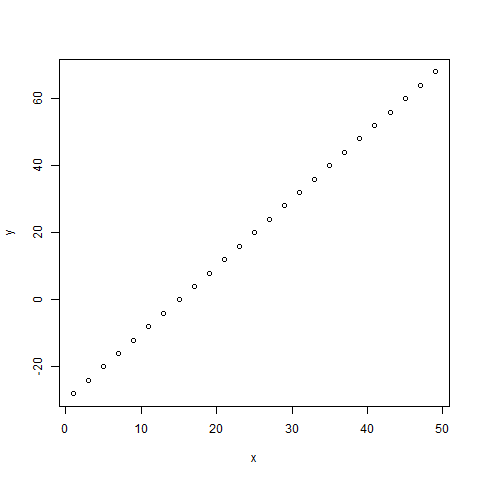
\includegraphics[width=0.35\columnwidth]{Abhishekplot}\centering
\caption{My first graph on Latex}
\end{figure}
\end{enumerate}
\section*{References}
\begin{itemize}
\item \texttt{Lectures and notes of Prof.M.M. Dalkilic}
\item \texttt{"Introduction to Data Mining" by Tan, Steinbach and Kumar}
\end{itemize}
\end{document}